\hypertarget{build-a-conversational-ai-system-with-jaseci}{%
\section{Build a Conversational AI System with
Jaseci}\label{build-a-conversational-ai-system-with-jaseci}}

In this tutorial, you are going to learn how to build a state-of-the-art
conversational AI system with Jaseci and the Jac language. You will
learn the basics of Jaseci, training state-of-the-art AI models, and
everything in between, in order to create an end-to-end fully-functional
conversational AI system.

Excited? Hell yeah! Let's jump in.

\hypertarget{preparation}{%
\subsection{Preparation}\label{preparation}}

To install jaseci, run in your development environment

\begin{lstlisting}
pip install jaseci
\end{lstlisting}

To test the installation is successful, run

\begin{lstlisting}
jsctl -- help
\end{lstlisting}

\passthrough{\lstinline!jsctl!} stands for the Jaseci Command Line
Interface. If the command above displays the help menu for
\passthrough{\lstinline!jsctl!}, then you have succssfully installed
jaseci.

\begin{quote}
\textbf{Note}

Take a look and get familiarized with these commands while you are at
it. \passthrough{\lstinline!jsctl!} will be frequently used throughout
this journey.
\end{quote}

\hypertarget{background}{%
\subsection{Background}\label{background}}

A few essential concepts to get familiar with.

\hypertarget{graph-nodes-edges}{%
\subsubsection{Graph, nodes, edges}\label{graph-nodes-edges}}

Refer to relevant sections of the Jaseci Bible.

\hypertarget{walker}{%
\subsubsection{Walker}\label{walker}}

Refer to relevant sections of the Jaseci Bible.

\hypertarget{automated-faq-answering-chatbot}{%
\section{Automated FAQ answering
chatbot}\label{automated-faq-answering-chatbot}}

Our conversational AI system will consists of multiple components. To
start, we are going to build a chatbot that can answer FAQ questions
without any custom training, using zeroshot NLP models. At the end of
this section, you will have a chatbot that, when given a question,
searches in its knowledge base the most relevant answer and return that
answer.

The use case here is a Tesla FAQ chatbot. We will be using the list of
FAQs from https://www.tesla.com/en\_SG/support/faq.

\begin{quote}
\textbf{Note}

This architecture works for any FAQ topics and use case. Feel free to
pick another product/website/company's FAQ if you'd like!
\end{quote}

\hypertarget{define-the-nodes}{%
\subsection{Define the Nodes}\label{define-the-nodes}}

We have 3 different type of nodes:

\begin{itemize}
\tightlist
\item
  \passthrough{\lstinline!root!}: This is the root node of the graph. It
  is a built-in node type and each graph has one root node only.
\item
  \passthrough{\lstinline!faq\_root!}: This is the entry point of the
  FAQ handler. We will make the decision on the most relevant answer at
  this node.
\item
  \passthrough{\lstinline!faq\_state!}: This node represents a FAQ
  entry. It contains a candidate answer from the knowledge base.
\end{itemize}

Now let's define the custom node types.

\begin{lstlisting}
node faq_root;
node faq_state {
    has question;
    has answer;
}
\end{lstlisting}

The \passthrough{\lstinline!has!} keyword defines nodes variables. In
this case, each \passthrough{\lstinline!faq\_state!} has a
\passthrough{\lstinline!question!} and \passthrough{\lstinline!answer!}.

\begin{quote}
\textbf{Warning}

The \passthrough{\lstinline!root!} node does not need explicit
definition. It is a built-in node type. Avoid using
\passthrough{\lstinline!root!} as a custom node type.
\end{quote}

\hypertarget{build-the-graph}{%
\subsection{Build the Graph}\label{build-the-graph}}

For this FAQ chatbot, we will build a graph like illustrated here:

\begin{figure}
\centering
\includegraphics{images/faq_1.png}
\caption{Architecture of FAQ Bot}
\end{figure}

The idea here is that we will decide which FAQ entry is the most
relevant to the incoming question at the
\passthrough{\lstinline!faq\_root!} node and then we will traverse to
that node to fetch the corresponding answer.

To define this graph architecture:

\begin{lstlisting}
// Static graph definition
graph faq {
    has anchor faq_root;
    spawn {
        // Spawning the nodes
        faq_root = spawn node::faq_root;
        faq_answer_1 = spawn node::faq_state(
            question="How do I configure my order?",
            answer="To configure your order, log into your Tesla account."
        );
        faq_answer_2 = spawn node::faq_state(
            question="How do I order a tesla",
            answer="Visit our design studio to place your order."
        );
        faq_answer_3 = spawn node::faq_state(
            question="Can I request a test drive",
            answer="Yes. You must be a minimum of 25 years of age."
        );

        // Connecting the nodes together
        faq_root --> faq_answer_1;
        faq_root --> faq_answer_2;
        faq_root --> faq_answer_3;
    }
}
\end{lstlisting}

Let's break down this piece of code.

We observe two uses of the \passthrough{\lstinline!spawn!} keyword. To
spawn a node of a specific type, use the \passthrough{\lstinline!spawn!}
keyword for:

\begin{lstlisting}
faq_answer_1 = spawn node::faq_state(
    question="How do I configure my order?",
    answer="To configure your order, log into your Tesla account.",
);
\end{lstlisting}

In the above example, we just spawned a
\passthrough{\lstinline!faq\_state!} node called
\passthrough{\lstinline!faq\_answer\_1!} and initialized its
\passthrough{\lstinline!question!} and \passthrough{\lstinline!answer!}
variables.

\begin{quote}
\textbf{Note}

The \passthrough{\lstinline!spawn!} keyword can be used in this style to
spawn many different jaseci objects, such as nodes, graphs and walkers.
\end{quote}

The second usage of \passthrough{\lstinline!spawn!} is with the graph:

\begin{lstlisting}
graph faq {
    has anchor faq_root;
    spawn {
       ...
    }
}
\end{lstlisting}

In this context, the \passthrough{\lstinline!spawn!} designates a code
block with programmatic functionality to spawn a subgraph for which the
root node of that spawned graph will be the
\passthrough{\lstinline!has anchor faq\_root!}.

In this block:

\begin{itemize}
\tightlist
\item
  We spawn 4 nodes, one of the type \passthrough{\lstinline!faq\_root!}
  and three are of the type \passthrough{\lstinline!faq\_state!}.
\item
  We connect each of the faq answer state to the faq root with
  \passthrough{\lstinline!faq\_root --> faq\_answer\_*!}.
\item
  We set the \passthrough{\lstinline!faq\_root!} as the anchor node of
  the graph. As we will later see, spawning a graph will return its
  anchor node.
\end{itemize}

\begin{quote}
\textbf{Warning}

An anchor node is required for every graph block. It must be assigned
inside the spawn block of the graph definition.
\end{quote}

\hypertarget{initialize-the-graph}{%
\subsection{Initialize the Graph}\label{initialize-the-graph}}

Similar to nodes, in order to create the graph, we will use the
\passthrough{\lstinline!spawn!} keyword.

\begin{lstlisting}
walker init {
    root {
        spawn here --> graph::faq;
    }
}
\end{lstlisting}

This is the first walker we have introduced so let's break it down.

\begin{itemize}
\tightlist
\item
  The walker is called \passthrough{\lstinline!init!}.
\item
  It contains logic specifically for the \passthrough{\lstinline!root!}
  node, meaning that the code inside the
  \passthrough{\lstinline!root \{\}!} block will run \textbf{only} on
  the \passthrough{\lstinline!root!} node. This syntax applies for any
  node types, as you will see very soon. Every Jac program starts with a
  single root node, though as you will later learn, a walker can be
  executed on any node though root is default if none is specified.
\item
  \passthrough{\lstinline!spawn here --> graph::faq!} creates an
  instance of the \passthrough{\lstinline!faq!} graph and connect its
  anchor node to \passthrough{\lstinline!here!} which is the node the
  walker is currently on.
\end{itemize}

\begin{quote}
\textbf{Note}

\passthrough{\lstinline!init!} can be viewed as similar to
\passthrough{\lstinline!main!} in python. It is the default walker to
run when no specific walkers are specified for a
\passthrough{\lstinline!jac run!} command.

\passthrough{\lstinline!here!} is a very powerful keyword. It always
evaluates to the specific node the walker is currently on. You will be
using \passthrough{\lstinline!here!} a lot throughout this tutorial.
\end{quote}

\hypertarget{run-the-init-walker}{%
\subsection{\texorpdfstring{Run the \texttt{init}
Walker}{Run the init Walker}}\label{run-the-init-walker}}

Now, let's run the init walker to initialize the graph. First put all
the above code snippet in a single jac file and name it
\passthrough{\lstinline!main.jac!}, including

\begin{itemize}
\tightlist
\item
  nodes defintion
\item
  graph definition
\item
  init walker
\end{itemize}

Run \passthrough{\lstinline!jsctl!} to get into the jaseci shell
environment:

\begin{lstlisting}[language=bash]
jsctl
\end{lstlisting}

Inside the \passthrough{\lstinline!jsctl!} shell,

\begin{lstlisting}[language=bash]
jaseci > jac dot main.jac
\end{lstlisting}

This command runs the \passthrough{\lstinline!init!} walker of the
\passthrough{\lstinline!main.jac!} program and prints the state of its
graph in DOT format after the walker has finished.
\href{https://graphviz.org/doc/info/lang.html}{The DOT language} is a
popular graph description language widely used for representing complex
graphs.

The output should look something like this

\begin{figure}
\centering
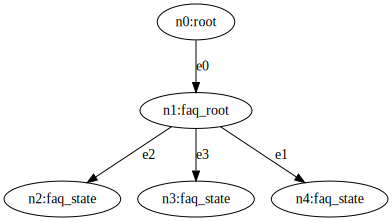
\includegraphics{images/dot_1.png}
\caption{Dot output for Faq graph}
\end{figure}

\begin{lstlisting}
strict digraph root {
    "n0" [ id="0955c04e4ff945b4b836748ef2bbd98a", label="n0:root"  ]
    "n1" [ id="c1240d79110941c1bc2feb18581951bd", label="n1:faq_state"  ]
    "n2" [ id="55333be285c246db88181ac34d16cd20", label="n2:faq_state"  ]
    "n3" [ id="d4fa8f2c46ca463f9237ef818e086a29", label="n3:faq_state"  ]
    "n4" [ id="f7b1c8ae82af4063ad53646adc5544e9", label="n4:faq_state"  ]
    "n0" -> "n1" [ id="a718fd6c938149269d3ade2af2eb023c", label="e0" ]
    "n1" -> "n2" [ id="3757cb15851249b4b6083d7cb3c34f8e", label="e1" ]
    "n1" -> "n4" [ id="626ce784a8f5423cae5d5d5ca857fc5c", label="e2" ]
    "n1" -> "n3" [ id="a609e7b54bde4a6a9c9711afdb123241", label="e3" ]
}
\end{lstlisting}

\begin{quote}
\textbf{Note}

We are not going to cover the DOT syntax. There are many resources
online if you are interested, e.g.,
https://graphviz.org/doc/info/lang.html
\end{quote}

\begin{quote}
\textbf{Note}

There are tools available to render a graph in DOT format. For example,
https://dreampuf.github.io/GraphvizOnline has as WSIWYG editor to render
dot graph in real time.
\end{quote}

Congratulations! You have just created your first functional jac
program!

\hypertarget{ask-the-question}{%
\subsection{Ask the Question}\label{ask-the-question}}

Alright, we have initialized the graph. Now it's time to create the code
for the question-answering. We will start with a simple string matching
for the answer selection algorithm. For this, we will create a new
walker called \passthrough{\lstinline!ask!}.

\begin{lstlisting}
walker ask {
    has question;
    root {
        question = std.input("AMA > ");
        take --> node::faq_root;
    }
    faq_root {
        take --> node::faq_state(question==question);
    }
    faq_state {:
        std.out(here.answer);
    }
}
\end{lstlisting}

This walker is more complex than the \passthrough{\lstinline!init!} one
and introduces a few new concepts so let's break it down!

\begin{itemize}
\tightlist
\item
  Similar to nodes, walker can also contain
  \passthrough{\lstinline!has!} variables. They define variables of the
  walker. They can also be passed as parameters when calling the walker.
\item
  \passthrough{\lstinline!std.input!} and
  \passthrough{\lstinline!std.out!} read and write to the command line.
\item
  This walker has logic for three types of node:
  \passthrough{\lstinline!root!}, \passthrough{\lstinline!faq\_root!}
  and \passthrough{\lstinline!faq\_state!}.

  \begin{itemize}
  \tightlist
  \item
    \passthrough{\lstinline!root!}: It simply traverse to the
    \passthrough{\lstinline!faq\_root!} node.
  \item
    \passthrough{\lstinline!faq\_root!}: This is where the answer
    selection algorithm is. We will find the most relevant
    \passthrough{\lstinline!faq\_state!} and then traverse to that node
    via a \passthrough{\lstinline!take!} statement. In this code
    snippet, we are using a very simple (and limited) string matching
    approach to try to match the predefined FAQ question with the user
    question.
  \item
    \passthrough{\lstinline!faq\_state!}: Print the answer to the
    terminal
  \end{itemize}
\end{itemize}

Before we run this walker, we are going to update the
\passthrough{\lstinline!init!} walker to speed up our development
process

\begin{lstlisting}
walker init {
    root {
        spawn here --> graph::faq;
        spawn here walker::ask;
    }
}
\end{lstlisting}

This serves as a shorthand so that we can initialize the graph and ask
question in one command.

\begin{quote}
\textbf{Note}

This demonstrates how one walker can spawn another walker using the
\passthrough{\lstinline!spawn!} keyword.
\end{quote}

Time to run the walker!

\begin{lstlisting}[language=bash]
jaseci > jac run main.jac
\end{lstlisting}

\passthrough{\lstinline!jac run!} functions very similarly to
\passthrough{\lstinline!jac dot!}, with the only difference being that
it doesn't return the graph in DOT format. Try giving it one of the
three questions we have predefined and it should respond with the
corresponding answer.

\hypertarget{introducing-universal-sentence-encoder}{%
\subsection{Introducing Universal Sentence
Encoder}\label{introducing-universal-sentence-encoder}}

Now, obviously, what we have now is not very ``AI'' and we need to fix
that. We are using the Universal Sentence Encoder QA model as the answer
selection algorithm. Universal Sentence Encoder is a language encoder
model that is pre-trained on large corpus of natural language data and
have been shown to be effective in many NLP tasks. In our application,
we are using it for zero-shot question-answering, i.e.~no custom
training required.

Jaseci has a set of built-in libraries or packages that are called
Jaseci actions. These actions cover a wide-range of state-of-the-art AI
models across many different NLP tasks. These actions are packaged in a
python module called \passthrough{\lstinline!jaseci\_kit!}.

To install \passthrough{\lstinline!jaseci\_kit!}:

\begin{lstlisting}[language=bash]
pip install jaseci_ai_kit
\end{lstlisting}

Now we load the action we need into our jaseci environment

\begin{lstlisting}[language=bash]
jaseci > actions load module jaseci_ai_kit.use_qa
\end{lstlisting}

Let's update our walker logic to use the USE QA model:

\begin{lstlisting}
walker ask {
    has question;
    root {
        question = std.input(">");
        take --> node::faq_root;
    }
    faq_root {
        answers = -->.answer;
        best_answer = use.qa_classify(
            text = question,
            classes = answers
        );
        take --> node::faq_state(answer==best_answer["match"]);
    }
    faq_state {
        std.out(here.answer);
    }
}
\end{lstlisting}

Even though there are only 5 lines of new code, there are many
interesting aspects so let's break it down!

\begin{itemize}
\tightlist
\item
  \passthrough{\lstinline!-->.answer!} collects the
  \passthrough{\lstinline!answer!} variable of all of the nodes that are
  connected to
  \passthrough{\lstinline!here!}/\passthrough{\lstinline!faq\_root!}
  with a \passthrough{\lstinline!-->!} connection.
\item
  \passthrough{\lstinline!use.qa\_classify!} is one of the action
  supported by the USE QA action set. It takes in a question and a list
  of candidate answers and return the most relevant one.
\end{itemize}

Now let's run this new walker and you can now ask questions that are
relevant to the answers beyond just the predefined ones.

\hypertarget{scale-it-out}{%
\subsection{Scale it Out}\label{scale-it-out}}

So far we have created a FAQ bot that is capble of provide answer in
three topics. To make this useful beyond just a prototype, we are now
going to expand its database of answers. Instead of manually spawning
and connecting a node for each FAQ entry, we are going to write a walker
that automatically expand our graph:

\begin{lstlisting}
walker ingest_faq {
    has kb_file;
    root: take --> node::faq_root;
    faq_root {
        kb = file.load_json(kb_file);
        for faq in kb {
            answer = faq["answer"];
            spawn here --> node::faq_state(answer=answer);
        }
    }
}
\end{lstlisting}

An example knowledge base file look like this

\begin{lstlisting}
[
  {
    "question": "I have a Model 3 reservation, how do I configure my order?",
    "answer": "To configure your order, log into your Tesla Account and select manage on your existing reservation to configure your Tesla. Your original USD deposit has now been converted to SGD."
  },
  {
    "question": "How do I order a Tesla?",
    "answer": "Visit our Design Studio to explore our latest options and place your order. The purchase price and estimated delivery date will change based on your configuration."
  },
  {
    "question": "Can I request a Test Drive?",
    "answer": "Yes, you can request for a test drive. Please note that drivers must be a minimum of 25 years of age and not exceeding 65 years of age, hold a full driving license with over 2 years of driving experience. Insurance conditions relating to your specific status must be reviewed and accepted prior to the test drive."
  }
]
\end{lstlisting}

Save the above json in a file named
\passthrough{\lstinline!tesla\_faq.json!} and make it is in the same
location as \passthrough{\lstinline!main.jac!}. Let's now update the
\passthrough{\lstinline!init!} walker. Because we are going to use the
\passthrough{\lstinline!ingest\_faq!} walker to generate the graph, we
won't need the static graph definition.

\begin{lstlisting}
walker init {
    root {
        spawn here --> node::faq_root;
        spawn here walker::ingest_faq(kb_file="tesla_faq.json");
        spawn here walker::ask;
    }
}
\end{lstlisting}

What we are doing here is

\begin{itemize}
\tightlist
\item
  Spawn a \passthrough{\lstinline!faq\_root!} node
\item
  Run the \passthrough{\lstinline!ingest\_faq!} walker to create the
  neccessary \passthrough{\lstinline!faq\_state!} nodes based on the
  question-answer entires in the
  \passthrough{\lstinline!tesla\_faq.json!} file.
\item
  Launch the \passthrough{\lstinline!ask!} walker
\end{itemize}

Let's run the program one more time and test it out!

\begin{lstlisting}[language=bash]
jaseci > jac run main.jac
\end{lstlisting}

\begin{quote}
\textbf{Note}

Try more varied questions. Now we have a longer answer with more rich
information, it has a higher coverage of information that will be able
to answer more questions.
\end{quote}

\begin{quote}
\textbf{Note}

If you are feeling adventurous, try downloading the complete list of
entires on the Tesla FAQ page and use it to create a production-level
FAQ bot. See if you can push the model to its limit!
\end{quote}

\hypertarget{next-up}{%
\section{Next up!}\label{next-up}}

\begin{figure}
\centering
\includegraphics{images/arch.png}
\caption{Full architecture of Tesla AI}
\end{figure}

Here is a preview on what's next to come in this journey!

On the right is the architecture diagram of the complete system we are
going to build. Here are the major components:

\begin{itemize}
\tightlist
\item
  Zero-shot FAQ (what we have built so far).
\item
  Action-oriented Multi-turn Dialogue System.
\item
  Training and inference with an intent classification model.
\item
  Training and inference with an entity extraction model.
\item
  Testing.
\item
  Deploying your Jac application to a production environment.
\item
  Training data collection and curation.
\end{itemize}
